\chapter{Proposed Methodology}
The methodology for this project integrates time-series prediction with real-time environmental sensing to optimize classroom ventilation. The main objective is to forecast occupancy and CO₂ levels using an LSTM (Long Short-Term Memory) model, which excels in handling time-dependent data. The system architecture is built around Arduino-based sensor nodes and a central Raspberry Pi, which together collect and process real-time data from classrooms. This data includes CO₂ concentration, temperature, humidity, and occupancy status, and is used to make smart predictions that inform decision-making. These predictions determine ventilation actions like activating cooling fans, triggering alerts, and displaying room status on LCD screens to guide users. The methodology is structured into four key phases: (1) dataset creation and preprocessing, (2) model development and training, (3) loss function and evaluation metric selection, and (4) prediction-based decision logic. These phases are closely integrated to establish a feedback loop where sensing, prediction, and system action continuously improve indoor air quality and user comfort in real time.
\section{Dataset and Preprocessing}
\\In any machine learning project, especially those involving time-series forecasting in dynamic, real-world environments like classrooms, the quality of the dataset and the preprocessing strategy form the foundation for model success. For this LSTM-based indoor air quality monitoring system, the dataset used was not simply picked from a single source—it was thoughtfully compiled, harmonized, and structured to reflect real-world classroom conditions as accurately as possible. Since the model’s core objective is to predict CO₂ levels and guide ventilation decisions, instead of relying on a single source, then carefully merged several open datasets from educational institutions, smart buildings, and air quality research projects. These sources gave us detailed, time-stamped readings of CO₂ concentrations (in ppm), temperature, humidity, and occupancy counts. Some of the data came from offices, others from classrooms, and many included varying room sizes and ventilation setups.

 The preprocessing phase played a vital role in transforming raw sensor readings into a clean and usable format suitable for LSTM training. Time-series data, by nature, can be messy. There were missing readings. Initially, addressed the issue of missing values through time-based interpolation, which filled gaps without disrupting the natural flow of the sequence data. Once the data was cleaned and normalized, the next step was to reshape it into a format suitable for LSTM training.Then chosed a sliding window approach, where the model observes the last 10–15 timesteps to predict the next one. This method of creating overlapping sequences allowed the model to see enough historical context to understand temporal trends, such as gradual CO₂ accumulation due to occupancy or ventilation improvements due to open windows or fans.Another important aspect of preprocessing was splitting the data into training, validation, and test sets.
 However, in time-series forecasting, it’s crucial not to shuffle the data before splitting, as it can destroy the temporal order, leading to unrealistic results. Maintained the chronological order and divided the dataset into 70\% training, 20\% validation, and 10\% testing. This allowed the model to learn from past patterns and be evaluated on unseen future data—closely simulating how the model would behave in a real classroom deployment.To make the model even more robust and added subtle variations during training by injecting a bit of noise into the sequences. This mimics real-world sensor differences and helps prevent overfitting. On the Raspberry Pi, and also implemented a harmonization technique where average the last few readings before making a prediction. This reduces the effect of sudden spikes and creates smoother, more reliable predictions.
\section{Model Building and training:}
\subsection{System Architecture}


\begin{figure}[h]
		\centering
	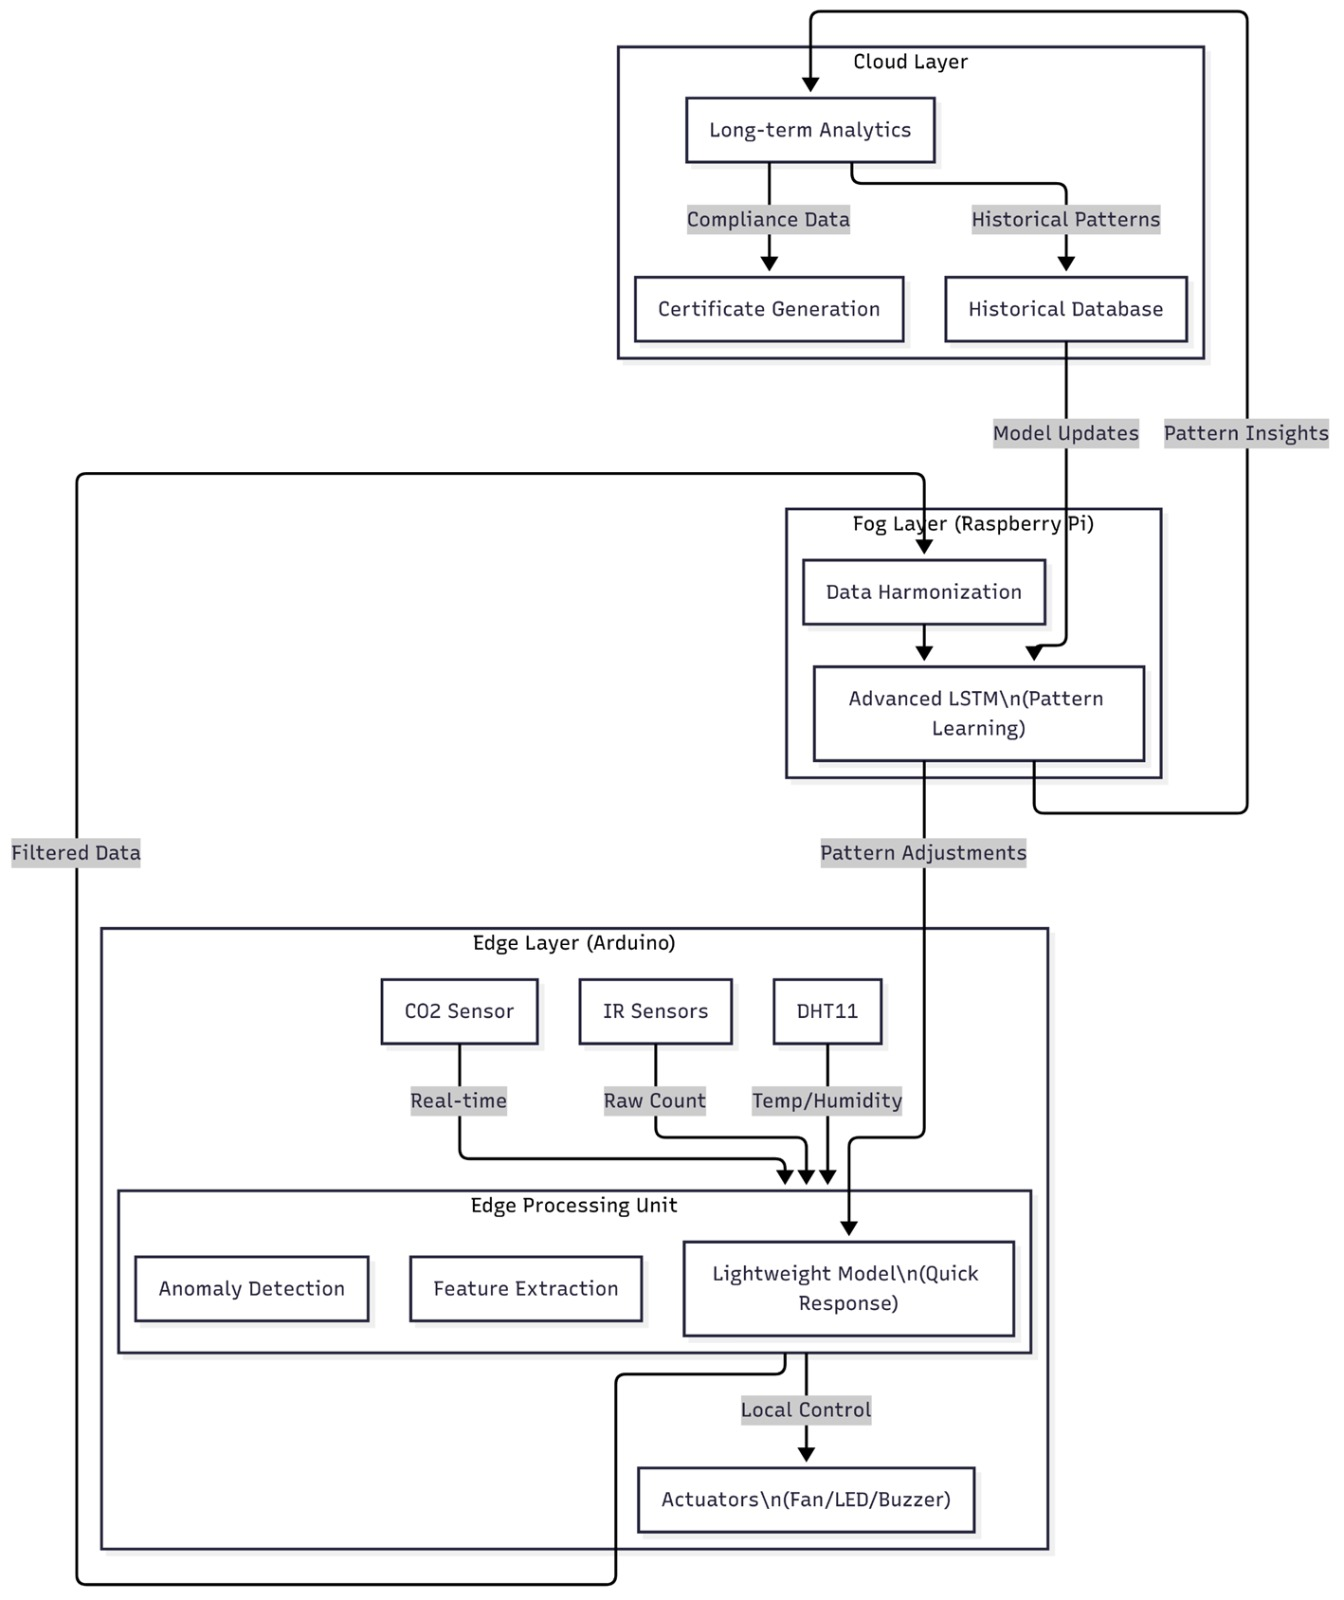
\includegraphics[width=1.0\textwidth]{Chapters/workflow.jpg (1).jpeg}
    \label{fig:augmentation}
		\caption{Proposed System Flow}
\end{figure}\\
The architecture of this system is built as a smart, multi-layered framework designed to intelligently manage classroom ventilation by predicting CO₂ levels and occupancy trends. It follows an Edge-Fog-Cloud computing model, where each layer has a specific role in creating a seamless, responsive environment. At the most immediate level, we have the Edge Layer, which includes Arduino-based setups installed in classrooms. These units are equipped with CO₂ sensors, IR sensors, and DHT11 sensors to collect real-time data on indoor air quality, occupancy, temperature, and humidity. The edge system doesn't just gather data—it also processes it locally. A lightweight program runs on the Arduino to detect sudden anomalies or high CO₂ spikes and instantly responds by activating connected devices like fans, LEDs, or buzzers. This ensures that urgent air quality issues can be addressed immediately, without waiting for higher-level analysis or cloud instructions.

Next, moving to the Fog Layer(\ref{fig:augmentation}), where a Raspberry Pi acts as a smarter, more powerful processing hub. It collects the refined data from the edge devices, aligns it, and feeds it into a pre-trained LSTM model. This model is capable of recognizing patterns over time, such as how occupancy and CO₂ levels typically change throughout the day. Based on these predictions, the Raspberry Pi can make informed decisions about room conditions—like selecting the better-ventilated room or preemptively starting ventilation. What's more, the fog layer can send feedback to the edge devices, helping improve their quick-response mechanisms over time. This creates a two-way interaction where learning flows both upward and downward, making the system more adaptive.

Finally, at the top, the Cloud Layer takes on the role of long-term storage and analysis. Data from the fog layer is sent to the cloud for deeper insights, such as trend discovery, historical analysis, and compliance tracking. One of the key functions of this layer is generating certificates to confirm whether classroom air quality standards are being met. The cloud also plays a vital role in updating the prediction models, sending improved versions back to the fog and edge systems to keep everything current and optimized. This architecture is not just a chain of data flow—it's a collaborative loop. The edge layer ensures quick, local action; the fog layer makes smarter decisions based on patterns; and the cloud drives long-term improvements and compliance. Each layer strengthens the others, creating a responsive, evolving system that intelligently manages classroom environments for comfort, safety, and health.
\textbf{LSTM model} address this problem by introducing a memory cell, which is a container that can hold information for an extended period. LSTM networks are capable of learning long-term dependencies in sequential data, which makes them well-suited for tasks such as language translation, speech recognition, and time series forecasting. LSTMs can also be used in combination with other neural network architectures, such as Convolutional Neural Networks (CNNs) for image and video analysis. The memory cell is controlled by three gates: the input gate, the forget gate, and the output gate. These gates decide what information to add to, remove from, and output from the memory cell. The input gate controls what information is added to the memory cell. The forget gate controls what information is removed from the memory cell. And the output gate controls what information is output from the memory cell. This allows LSTM networks to selectively retain or discard information as it flows through the network, which allows them to learn long-term dependencies.\\


At the heart of this intelligent classroom monitoring system lies a predictive deep learning model designed specifically to understand how indoor environmental factors evolve over time. To achieve this, employed a Long Short-Term Memory (LSTM) neural network—an advanced type of recurrent neural network (RNN) that excels at recognizing temporal dependencies in sequential data. LSTM is particularly suitable for task because it retains long-term contextual information and avoids the vanishing gradient problem that limits traditional RNNs. The model is designed to process and learn from four primary environmental inputs: CO₂ concentration, temperature, humidity, and occupancy count. These values are gathered in real-time and represent the immediate environmental state of the classroom. The architecture begins with an input layer that accepts a sequence of these features over multiple timesteps (e.g., the last 10–15 readings).

The core architecture consists of two stacked LSTM layers. The first LSTM layer has 64 hidden units, which helps it capture complex patterns across long sequences. This is followed by a second LSTM layer with 32 units, allowing the network to refine those patterns into more actionable representations. Between these layers, Dropout regularization is applied to prevent overfitting. Dropout randomly disables a fraction of the neurons during training, encouraging the model to learn more generalized features, especially useful given the real-world nature and limited size of the dataset. Following the LSTM layers, the network connects to a Dense (fully connected) layer, which condenses the temporal feature output into a single scalar value: the predicted CO₂ concentration for the next time step. This simple output allows the system to take quick, interpretable actions based on a single decision point.

The model is compiled using the Mean Squared Error (MSE) as the loss function. MSE is ideal for regression tasks like ours, where the goal is to minimize the gap between predicted and actual CO₂ values. For optimization, the Adam optimizer is used. Adam is a widely used and efficient optimizer that adapts the learning rate during training, promoting faster convergence and better generalization. The final architecture is intentionally lightweight and efficient, designed with edge deployment in mind. Once training is complete, the model is saved as pretrained$_$lstm.weights.h5, and the associated data scaler is stored as pretrained$_$scaler.joblib. These components are later used on the Raspberry Pi to enable real-time predictions, ensuring that the model does not have to be retrained in the field.
\\

\subsection{Training Process}
The training process follows a well-structured and iterative workflow designed to build a stable, reliable forecasting model. It begins with preprocessing the data into sequences using a sliding window method. This means that for every prediction, the model is fed with data from the last 10–15 time steps. Each training sample, therefore, becomes a snapshot of recent environmental trends, allowing the model to learn how conditions evolve. The data is normalized using Min-Max scaling, ensuring consistent feature contribution and preventing skew from variables like CO₂ values (which can range up to 2000 ppm) compared to occupancy (which typically ranges between 0–30). These sequences are then divided into training, validation, and testing sets, preserving their chronological order to maintain the time-based integrity of the dataset.

The model is trained over 200 epochs using a batch size of 32. To prevent overfitting and reduce training time, EarlyStopping is applied, which halts training once the validation loss plateaus. Additionally, a learning rate scheduler is integrated to adjust the learning rate dynamically based on performance feedback, improving convergence and helping the model avoid local minima.Model performance is continuously evaluated using, Mean Square Error (MSE)measures the average squared difference between actual and predicted value.

Our best-trained model achieved well within operational requirements for indoor air quality control. This level of precision enables the system to make confident decisions on whether to trigger ventilation or maintain current conditions.After training, the model is converted into a lightweight format using TensorFlow Lite, making it suitable for edge devices with limited processing power, such as the Raspberry Pi 4. This deployment approach ensures that predictions are made locally—without reliance on the cloud—allowing for low-latency, privacy-preserving, and reliable operation even in offline environments.

 This architecture and training pipeline not only leverage the strengths of deep learning in modeling time-dependent data but also demonstrate careful attention to real-world deployment challenges. The LSTM model's predictive power enables proactive air quality management, while its efficient design ensures smooth real-time integration with embedded hardware. Together, they form the intelligent “brain” of the classroom monitoring system—anticipating problems before they arise and guiding timely, energy-efficient responses.

\section{Loss Function and Evaluation Metrics}
When building a model that predicts how environmental conditions like CO₂ levels change over time, one of the most important steps is choosing how to measure the model’s learning. In machine learning, this is done using a loss function, which acts like a compass, guiding the model as it learns to make better predictions. In this project—where the goal is to forecast indoor CO₂ concentrations accurately within a classroom setting  the Mean Squared Error (MSE) selected as the main loss function. MSE is widely used in regression problems and is especially effective when we want to minimize large errors, which can be critical in systems that control real-world operations like ventilation.

The idea behind MSE is simple it calculates how far off the model’s predictions are from the actual values, squares those errors (to punish larger mistakes more heavily), and then averages them out. This squaring effect means that even a moderate prediction error can carry weight in the learning process. That’s exactly what we need in a ventilation system—if CO₂ predictions are too far off, the system might react too late or take unnecessary action. By minimizing MSE, we help the model focus on staying as close as possible to the actual environmental conditions. In this system, we use a combination of loss functions and evaluation metrics to train and assess the LSTM model's performance in forecasting indoor CO₂ levels. MSE measures the average squared difference between actual and predicted values. It is defined as(\ref{eq:mse})


\begin{equation}
\mathcal{L}_{\text{MSE}} = \frac{1}{N} \sum_{i=1}^{N} (y_i - \hat{y}_i)^2
\label{eq:mse} 
\end{equation}

The classroom monitoring system primarily employs Mean Squared Error (MSE) as its fundamental loss function, implemented through the PyTorch framework. This choice is particularly significant for the multi-parameter environmental monitoring task. The MSE calculation in the system processes multiple environmental variables simultaneously, including CO2 levels, temperature, humidity, and occupancy. In the implementation, MSE is calculated using PyTorch's built-in MSELoss criterion, as evidenced by the code line 'criterion = nn.MSELoss()'. This loss function squares the difference between predicted and actual values for each parameter, effectively penalizing larger prediction errors more heavily than smaller ones. The squaring operation ensures that the model pays special attention to significant deviations in environmental parameters, which is crucial for maintaining optimal classroom conditions. The MSE implementation in this system is particularly effective because it provides a single, comprehensive error metric that accounts for all monitored environmental parameters simultaneously.(\ref{eq:mse})







\section{Feature Engineering for Air Quality Prediction}

In smart ventilation systems, particularly in academic environments like classrooms, maintaining healthy air quality is crucial not only for comfort but also for productivity and overall well-being. To achieve this, the project introduces a key performance metric known as KPIv (Key Performance Indicator for Ventilation), which is used to quantify the ventilation quality of a room in real time. This value provides a compact yet comprehensive insight into how well-ventilated a classroom is, taking into account real-time sensor inputs and estimated occupancy. The KPIv is designed to be both responsive and interpretable. Its value ranges based on CO₂ concentration and occupancy-related inputs. When CO₂ levels exceed 1000 ppm, which is generally accepted as a threshold for poor air quality, the KPIv is set to the maximum value of 2.0, indicating that the room requires immediate ventilation. On the other hand, when CO₂ is below this threshold and actual occupancy is recorded, a more nuanced computation is used that factors in both the number of people present and the CO₂ buildup. In such cases, KPIv is calculated using the following formula(\ref{eq:KPIv})

\begin{equation}
KPIv = 
\begin{cases} 
2.0 & \text{if } CO_2 > 1000 \, \text{ppm} \\
\frac{CO_2 - 400}{20 \times actual\_people} & \text{if } actual\_people > 0 \\
0.5 & \text{if } estimated\_people > 0 \text{ and } actual\_people = 0 \\
0.0 & \text{otherwise}
\end{cases}
\label{eq:KPIv}
\end{equation}

This structure ensures that the metric remains robust even in cases where sensor discrepancies arise. For instance, if estimated people (e.g., from a camera or motion detector) is greater than zero but actual people (from, say, a seat sensor) is zero, the KPIv is set to 0.5—a moderate value that warns of potential sensor error or unnoticed occupancy. If neither estimated nor actual presence is detected, KPIv defaults to 0.0, indicating no ventilation demand. Beyond KPIv, the system also calculates a Room Quality Score, which offers a more comprehensive assessment of classroom air quality by incorporating multiple environmental variables. This score is determined using the formula(\ref{eq:Score})
\begin{equation}
    Score = 5 \times KPIv + 0.2 \times |Temperature - 24| + 0.3 \times \frac{CO_2}{1000} + 0.1 \times Occupancy
    \label{eq:Score}
\end{equation}
Here, KPIv carries the most weight, reflecting its critical role in evaluating ventilation. Temperature is normalized around an ideal of 24°C, while CO₂ and occupancy are factored in to represent discomfort and population density. This scoring system enables institutions to monitor air quality at scale, prioritize ventilation in problem areas, and even automate decisions like triggering exhaust fans or notifications. Altogether, the combination of KPIv and Room Quality Scoring bridges sensor data with actionable intelligence, helping maintain a safe and healthy learning environment while also enabling data-driven building management strategies.


